\section{Methods}

\subsection{Distance metrics}

The following sections describe a range of different types of distance metrics,
that is, methods for measuring the distance between sequences.

\subsubsection{Edit distance}

One type of \emph{edit distance} is the \emph{Levenshtein}
distance~\cite{levenshtein}, which is a string metric for determining the
similarity between two sequences. It is defined to be the minimum number of
edits to transform the first sequence into the other.~\cite[p.~52]{dong}

The edit operations consists of \emph{insertions}, \emph{deletions} and
\emph{substitutions}. These operations are, respectively, inserting a letter,
removing a letter and changing one letter into another.

For example, the two sequences
\begin{center}
  \texttt{ACGT} \\
  \texttt{ACGGC}
\end{center}
would have a distance of 2 (substituting T for G and inserting a C). However,
there are some cases where the relevance of the distance is arguable. Consider
the sequences
\begin{center}
  \texttt{AACC} \\
  \texttt{CCAA}
\end{center}
with a distance of 4. The two sequences actually have the maximal distance
possible even though one is just a rotation of the other and in a biological
context, one might want this to results in a low distance, e.g. for gene
sequences that are split up and rejoined in different order.

%A naive version of the Levenshtein distance metric was implemented, but as
%expected, this is absolutely useless in any practical setting, since it does
%not reuse already calculated results. Therefore, this was quickly transformed
%into a dynamic programming solution, which solves subproblems just once, stores
%and reuses the intermediate results. This dynamic programming bottom up
%solution was however still very slow, yielding a performance of around 70
%comparisons per second.

A bottom-up dynamic programming version of the Levenshtein algorithm was
implemented and tested on real DNA/RNA data to evaluate its performance, and it
was clear that this algorithm was not suitable for large data sets, because it
would be infeasible to complete even a linear time clustering of the data using
this distance metric. The implementation could most likely be optimized
further, but because of the characteristics of an edit distance algorithm like
Levenshtein and because of the performance requirements for this project, it
was decided to not pursue further optimization and instead focus on other types
of algorithms. Furthermore, the Levenshtein distance penalizes rotations, i.e.
it results in an increased distance.

The Levenshtein distance can still be used for evaluation and benchmarking
against other metrics. The algorithm is attached in appendix
\ref{app:levenshtein_algorithm} and results from tests are shown in section
\ref{sec:results}.

As stated in \cite[pp.~1-2]{andoni}, ``The worst-case running time known for
this problem has not improved in three decades (..)'', specifically it states
that the running time of Levenshtein is $O(d^2)$, where $d$ is the length of
the two sequences, and $O(d^2/\log_2(d))$ for a constant size alphabet. It
further supports the conclusion that the running time of the Levenshtein
algorithm is too poor for the large data sets of the problem domain.

This lack of improvements of the performance of edit distance is one motivation
for the introduction of the concept of sequence alignment.

%The implemented dynamic programming solution has a running time of $O(nm)$,
%where $n$ and $m$ are the lengths of the sequences, and this running time seems
%to be inherent in this approach to measuring distance between sequences, as it
%needs to consider all possible edits to one sequence for each position in the
%other sequence.


\subsubsection{Sequence alignment}

\emph{Sequence alignment} is used in bioinformatics to identify regions of
similarity by aligning the characters of two or more sequences in a certain
manner. Besides shifting a sequence to a side, gaps can be inserted between
characters as well. We represent a gap with '-' and it indicates an insertion
in one sequence or a deletion from another sequence.~\cite[pp.~135-136]{dong}

We call a column that includes '-' for an \emph{indel}, which is a contraction
of the first letters from insertion and deletion. If it does not and all
characters in the column are same, then we have a match. Otherwise, it is a
mismatch.

\begin{figure}[H]
  \centering
  \verb+ATGCAACGA+ \\
  \verb+ |||  |||+ \\
  \verb+-TGCG-CGA+
  \caption{Sequence alignment of `ATGCAACGA' and `TGCGCGA'}
  \label{fig:seqAlignment}
\end{figure}

Figure \ref{fig:seqAlignment} displays an alignment of two sequences. In column
0 is an indel, in columns 1-3 are matches, in column 4 is a mismatch and so
forth. The vertical bar characters in the middle line, indicates matches. The
number of each type can then be used in a formula to calculate the similarity
between the sequences. Note that more than two sequences can be aligned in a
\emph{multiple sequence alignment}.

There are many alignments. Among those is an optimal alignment which is the one
that is searched for.

Both \texttt{UCLUST} and the very recent project \texttt{VSEARCH} uses some
kind of sequence alignment for comparing sequences. \texttt{VSEARCH} uses a
parallelized version of the dynamic programming algorithm Needleman-Wunsch,
while \texttt{UCLUST} uses a heuristic procedure by default, but can be
instructed to use full dynamic programming with either the Needleman-Wunsch or
Smith-Waterman algorithm. However, this will make \texttt{UCLUST} much
slower.~\cite{vsearch} The heuristic algorithm used in \texttt{UCLUST} gives an
approximation of the optimal alignment for the purpose of increased
performance, but the alignment is not guaranteed to be optimal.

As opposed to \texttt{USEARCH}, \texttt{VSEARCH} is free and open-source
software and is designed for 64-bit processors, so it does not have the
limitation on usable memory that the free, 32-bit version of \texttt{USEARCH}
has.

Sequence alignment is still a computationally expensive operation and for
comparison of sequences with low similarity, the results of sequence alignment
are often poor. Additionally, as with the Levenshtein distance metric, sequence
alignment is very sensitive to the ordering of parts of sequences.
\emph{Alignment-free} sequence comparison methods strive to provide a measure
of sequence similarity while avoiding the costly computation that alignment
involves. Alignment-free comparison allows one to look at each of the sequences
independently, extracting some characteristics, or \emph{features}, of the each
sequence and then comparing these characteristics.  This can possibly reduce
the complexity of the comparison to linear time or better. One such
alignment-free method, is $k$-mer counting which will be presented and analyzed
in the following section.


\subsubsection{Feature based distance}

A $k$-mer, or $k$-gram or simply a \emph{word}, is a sequence of length $k > 0$
over some alphabet $\mathcal{A}$ of a sequence. An interesting feature of a
sequence is which $k$-mers occur in that sequence and how many times they
occur. Thus, \emph{$k$-mer counting} and similar metrics are \emph{feature
based distance metrics}.

$d2$ is a feature based distance metric, using $k$-mers as the feature. The
distance is calculated by counting the $k$-mers occurring in two sequences,
representing these occurrences as two vectors and finally taking the Euclidean
distance between these two vectors.~\cite[pp.~53-54]{dong}

Let $c_x(w)$ be the number of times that a $k$-mer $w$ occurs in the sequence
$x$. Then the $d2$ distance between two sequences, $x$ and $y$, can be defined
as follows~\cite[pp.~1-2]{hazelhurst}:
\begin{equation}
  d2_k(x,y) \eqdef \sqrt{\sum_{w \in K(x) \cup K(y)} (c_x(w) - c_y(w))^2}
\end{equation}
where $K(x)$ and $K(y)$ denotes the set of $k$-mers in $x$ and $y$,
respectively.

As an example, the two $2$-mer frequency vectors of the sequences
\begin{align*}
  S_1 &= AGACTG \\
  S_2 &= ACAGAT
\end{align*}
over the alphabet $\mathcal{A} = \{A,C,T,G\}$, can be illustrated as follows:

\begin{table}[!h]
\centering
\scalebox{0.75}{
\begin{tabular}{c | c c c c c c c c c c c c c c c c}
        & AA & AC & AG & AT & CA & CC & CG & CT & GA & GC & GG & GT & TA & TC & TG & TT \\
  \hline
  $S_1$ &    &  1 &  1 &    &    &    &    &  1 &  1 &    &    &    &    &    &  1 &    \\
  \hline
  $S_2$ &    &  1 &  1 &  1 &  1 &    &    &    &  1 &    &    &    &    &    &    &    \\
\end{tabular}}
\end{table}

The Euclidean distance would then be calculated as
\begin{align*}
  d2_2(S_1, S_2)
    &= \sqrt{(1-1)^2 + (1-1)^2 + (-1)^2 + (-1)^2 + 1^2 + (1-1)^2 + 1^2} \\
    &= 2
\end{align*}

The first version of the $d2$ distance metric algorithm descibed above, is
shown in figure \ref{alg:d2_basic} and it has been implemented as well. This
algorithm maintains a single frequency vector, as a map structure to allow for
large $k$ which results in a large number of possible different $k$-mers. The
map is indexed using the lexicographical position of the $k$-mer. When
iterating through the first sequence, $k$-mer counts are incremented and when
iterating through the second sequence, they are decremented. Finally all the
frequencies are squared and the square root of the sum is returned,
corresponding to the Euclidean distance between frequency vectors for the two
sequences.

\begin{algorithm}
  \caption{Basic \textsc{d2} distance metric}
  \label{alg:d2_basic}
  \begin{algorithmic}[1]
    \Require{$s$ and $t$ are DNA or RNA sequences and $k \in \mathbb{Z}^+$}
    \Statex
    \Function{d2}{$s, t, k$}
      \State initialize \texttt{freq\_map}
      \For{$i \gets 0$ to $length(s) - k$}
        \State freq\_map[index\_of\_kmer(s.substring(i, k)]\texttt{++}
      \EndFor
      \For{$i \gets 0$ to $length(t) - k$}
        \State freq\_map[index\_of\_kmer(t.substring(i, k)]\texttt{--}
      \EndFor
      \State $total \gets 0$
      \ForAll{$e \in$ freq\_map}
        \State $total \gets e.value^2$  \Comment{calculate the Euclidean distance}
      \EndFor
      \State \Return $\sqrt{total}$
    \EndFunction
  \end{algorithmic}
\end{algorithm}

To better support the measurement of distance between two sequences of
different length, but similar substrings, the concept of a \emph{window} can be
introduced. In this context, a window is a conceptual construction which gives
a view of fixed length substrings of two sequences. This window can then be
moved step by step over the two sequences, calculating the distance for each
position of the window and then using the lowest of those distances as the
resulting distance. In this way two sequences, where one is a prefix or postfix
of the other, will have zero distance. This concept is illustrated in figure
\ref{fig:d2_window_concept} where the blue box corresponds to the window, which
in this case has the length 10.

\begin{figure}[H]
\centering
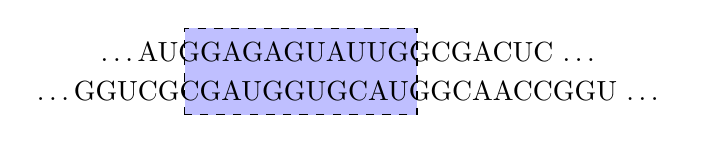
\begin{tikzpicture}
  \draw [fill=blue!25,dashed] (0,0.7) rectangle (2.95,1.8);
  \node at (2.1,1.5) {\dots AUGGAGAGUAUUGGCGACUC \dots};
  \node at (2.1,1.0) {\dots GGUCGCGAUGGUGCAUGGCAACCGGU \dots};
\end{tikzpicture}
\caption{Illustration of the concept of a window.}
\label{fig:d2_window_concept}
\end{figure}

The second, and current, version of the $d2$ distance function uses this
concept of a window, which is of length equal to the shortest of the two
sequences being compared. The distance in the first window calculated using the
basic \textsc{d2} algorithm described above, i.e. the distance between the
shortest of the two sequences and the first substring of the same length of the
longer sequence.

The window then iterates over the longer sequence and calculates the new
distance between the substring of the longer sequence and the shorter sequence.
This calculation is done using a kind of forward differences method for
reducing the calculations to a few fixed operations for calculating the
distance in the next window from the distance in the current window. This
concept is described in \cite{hazelhurst}.

The algorithm presented here uses a window size equal to the length of the
shortest of the two sequences. Let $|s|$ be the length of the shortest of the
two sequences. To begin with the, the $k$-mers in the first $|s|$ characters of
each sequence are counted and the \emph{Manhattan} distance between these two
frequency vectors is calculated.

The Manhattan distance is simply the Euclidean distance where squaring is
replaced with absolute value and the square root is omitted, i.e. for
$u, v \in \mathbb{Z}^n$,

\begin{equation}
  d_{Manhattan} \eqdef \sum_{i=1}^{n} |u_i - v_i| \;.
\end{equation}

This distance is the distance between the subsequences in the first position of
the window. To calculate the distance in the following window, i.e. advancing
the window through the longer of the two sequences by one character, it is
decided which $k$-mers exit and enter the window, respectively, and then by
looking at whether the existing $k$-mer count in the frequency vector is
negative or positive, it can be decided whether the distance increases or
decreased by 2 or whether it stays the same. Subsequently, the frequency vector
is updated to reflect the change in the new window. The following illustrates
the idea of a window and $k$-mers exiting and entering the window:

\begin{verbatim}
      |---- window ----------|
      ACTGATCGTAGCTAGCTAGTGTTG
      ACGTAGATCGTGGATGGCTGATCGTAGCTAAGCTTAGCTGATCG.....
      ^^^^                 ^^^^
      k-mer exiting        k-mer entering
\end{verbatim}

The Manhattan distance can be hard to use in practice, because it is very
dependent on the length of the shortest sequence (the length of the window),
the concept of the \emph{Jaccard index}~\cite{jaccard1901,jaccard1912}, or the
\emph{Jaccard similarity coefficient}, is used to ``normalize'' the distance to
a value in the interval $[0,1]$.

The Jaccard index of two sets $A$ and $B$ is defined as follows:
\begin{equation}
  J(A, B) \eqdef \frac{|A \cup B| - |A \cap B|}{|A \cup B|}
\end{equation}
 % TODO:  maybe actually Jaccard distance

In the context of $k$-mer frequencies, the union can be interpreted as the
total number of $k$-mers in the window in the two sequences, and the
intersection as the Manhattan distance in the window.


\subsection{Cluster analysis algorithms}

\subsubsection{Hierarchical clustering}

There are typically two types of hierarchical algorithms, both of which are
merge based, the agglomerative that works in a bottom-up manner and the
divisive that has a top-down approach, but we focus on explaining the
agglomerative. The agglomerative works in a bottom-up manner where all
sequences start as leaves. These sequences are considered clusters. They are
then merged together with the closest clusters until there is only one cluster
left. Alternatively, if the clustering is based on a similarity threshold, it
merges clusters until no more clusters can be merged.

% TODO: MAKE ILLUSTRATION

This addresses the question of what is required for a cluster to be close to another.
Besides measuring similarity between sequences with some distance
metric, a definition for when clusters should be merged is needed.

With the \textit{single-linkage} approach, only a sequence from both clusters
need an identity above the similarity threshold.  In the
\textit{complete-linkage} approach, all sequences from one cluster must be
above the threshold of all sequences from the other.  In the
\textit{average-linkage}, the average distance of all sequence pairs is
required to be above the threshold.

The singly-linkage approach is often used in sequence clustering though it has
its disadvantages as argued in \cite[pp. 62-63]{dong}.

\subsubsection{Graph based clustering}

TODO: Add short description of graph based clustering methods. % TODO


\subsubsection{Greedy algorithm like in \texttt{UCLUST}}
The \texttt{UCLUST} algorithm is greedy and is developed so that all member
sequences have similarity $\geq$ $T$ to their centroid.  It works by processing
one sequence at a time and comparing these to the existing centroids. If a
match is found, the sequence is assigned to the matching centroid, otherwise it
becomes a centroid of a new cluster.

It is designed to also support that each centroid has a similarity $<T$ to all
other centroids, but this is not guaranteed to hold. The reason is that the
algorithm only compares a sequence to a prespecified number of centroids given
by the \texttt{-maxrejects} parameter.

It uses the $k$-mer counts to locate centroid candidates for a match, though
how it does it is not very well described.

The similarity calculations are performed with global sequence alignments as
\cite{usearch} claims that using the word counts to calculate identity is not
sensitive enough.

%TODO? \subsubsection{Greedy algorithm with recalculation of centroids}

% Background: theoretical overview of the field of clustering
%   TODO: Clustering "history"





\subsection{Naive, greedy clustering algorithm}

A very simple, naive, greedy clustering algorithm has been implemented and will
be described briefly in this section. For the sake of convenience, it will be
referred to as \textsc{Naive\_Clust}.

Given a list of sequences and an initially empty list of centroids, the
algorithm works by iterating through the sequences and for every sequence, it
iterates through the list of centroids until a match is found or until the end
of the list. If a match is found, the sequences is added to the cluster
represented by the matching centroid, and otherwise the sequences becomes a new
centroid and is appended to the end of the list of centroids.

% TODO: complexity of algorithm
% This running time of this algorithm depends on the number of clusters in the
% output and therefore it might be around $O(c^2)$, where $c$ denoted the
% number of sequences, in the worst case where the number of clusters is equal
% to the number of sequences.  %O(k*(k-1)/2)

% TODO: refer to algorithm and implementation

This approach is not very useful in practice since it is very computationally
expensive in the worst case. The running time of the algorithm is very
dependent on the ordering of the sequences since the centroids will be in the
same order as in the list of sequences (i.e. the list of centroids is a
subsequence of the list of sequences) and if the first number of sequences
happens to be good centroids, which will match a lot of sequences, the
algorithm will perform good since the search for a centroid will end very
early. However, if the first number of sequences happens to be very dissimilar
from the rest of the data, then these will be compared against on every
iteration even though they might potentially never match anything.

Thus, there is a motivation to try and create more structure in the collection
of centroids, improve the search for a centroid to compare with the query
sequence or improving the ordering of the centroids.

% The problem with this approach is that it is potentially very computationally
% expensive to possible traverse the entire list of centroids for each
% iteration

% TODO: maybe mention the reason for introducing max_rejects


\subsection{\textsc{Simple\_Clust} algorithm}

Another clustering algorithm, named \textsc{Simple\_Clust}, was developed and
implemented, and will be described in this section. \textsc{Simple\_Clust}
tries to address some of the problems with the \textsc{Naive\_Clust} algorithm
by imposing more structure on the collection of centroids and by giving up
after some fixed number of comparisons of a given query sequence.

% We have developed a clustering algorithm, named \textsc{Simple\_Clust}
% (Algorithm \ref{alg:simple_clust}), which will be described in this section.

\textsc{Simple\_Clust} works by iterating sequentially through the sequences to
be clustered; the $max\_reject$ most frequent $k$-mers for the query sequence
are calculated and for each of these most frequent $k$-mers, a centroid which
has that $k$-mer as the most frequently occurring one (if one such centroid
exists) is compared with the query sequence to check if similarity their is
above the given threshold. The query sequence is assigned to the cluster for
the first centroid that matches the query sequence; if no such centroid is
found, out of the maximum possible $max\_reject$ number of tries, the query
sequence becomes a centroid for a new cluster and is added to the collection of
centroids along with the information about the most frequenty occurring $k$-mer
in the sequence.  % This is repeated for all sequences in the input file.

% the most frequent $k$-mer is decided and the sequence, along with this
% information, is added to the collection of centroids.

Algorithm \ref{alg:simple_clust} shows pseudocode for the
\textsc{Simple\_Clust} algorithm.

\begin{algorithm}
  \caption{\textsc{Simple\_Clust}}
  \label{alg:d2_naive}
  \begin{algorithmic}[1]
    \Require{$S$ is an array of [DR]NA sequences, $k \in \mathbb{Z}^+$ and
             $max\_rejects \in \mathbb{Z}^+$, $id \in [0,1]$}
    \Statex
    \Function{Simple\_Clust}{$S, k, max\_rejects$}
      \State $cluster\_count \gets 0$
      \State $centroids \gets []$ \Comment{map from $k$-mer to sequence}
      \ForAll{$s \in S$}
        \State $mfk \gets$ $max\_rejects$ most frequent $k$-mers in $s$
        \ForAll{$m \in mfk$}
          \If{$centroids[m]$ does not exists}
            \State continue
          \ElsIf{$distance(s, centroids[m]) \geq id$}
            \State add $s$ to cluster with centroid $centroids[m]$
            \State break
          \EndIf
        \EndFor
        \If{matching centroid was not found}
          \State centroids.insert(mfk[0], s)
        \EndIf
      \EndFor
      \State \Return $cluster\_count$
    \EndFunction
  \end{algorithmic}
  \label{alg:simple_clust}
\end{algorithm}


This algorithm did not perform as well as hoped, in particular for larger $k$
the number of different possible $k$-mers increases exponentially and for e.g.
$k = 6$ and a four letter alphabet, there are $4^6 = 4096$ different $k$-mers
and therefore the lookup in line 7 will likely often be unsuccessful.
Additionally, the most frequently occurring $k$-mer did not appear to be a
sufficiently good characteristic for choosing a centroid that is likely to
match, as is seen from the evaluation in section \ref{sec:results}. I.e. the
correspondence between the most frequently occurring $k$-mer of two sequences
and the similarity of the sequences, is evidently not very strong.  % TODO


\subsection{\textsc{Prioritized\_Intersect\_Clust}}

This section describes another clustering algorithm that has developed and
implemented, named \textsc{Prioritized\_Intersect\_Clust}, which looks at the
set of $k$-mers occurring in the query and target sequences and bases the
decision of whether to try comparing or not, on the cardinality of the
intersection between these sets. This way, the search for a likely match is not
just determined by the single most frequently occurring $k$-mer, as with
\textsc{Simple\_Clust}, but rather all the occurring $k$-mers, regardless of
their count. Additionally, the centroids are stored in a doubly linked list and
whenever a centroid matches a sequence, that centroid is moved to the front of
the list. This makes the algorithm less sensitive to the ordering of the input
sequences. The choice of the centroids will still be made greedily though, in
lack of well-performing alternatives, but the algorithm should nonetheless be
less prone to bad performance caused by an unlucky ordering of the input
sequences.

The idea of moving a matching centroid to the front of the list is, among other
things, inspired by the observation that the results from \texttt{UCLUST} and
\texttt{VSEARCH} often contain a large number of very small clusters and even
singleton clusters, i.e. clusters consisting of just a single sequence. For
example, clustering the data set \texttt{SILVA\_119\_SSURef\_tax\_silva.fasta}
with \texttt{USEARCH} and a similarity threshold of $0.95$, gives 117,205
clusters out of which 67,410 clusters are singleton clusters, that is more than
half of the clusters. These results are shown in listing \ref{fig:uclust_silva}
in section \ref{sec:results}.

\begin{algorithm}
  \caption{\textsc{Prioritized\_Intersect\_Clust}}
  \label{alg:prioritized_intersect_clust}
  \begin{algorithmic}[1]
    \Statex
    \State TODO: add pseudocode % TODO
  \end{algorithmic}
  \label{alg:simple_clust}
\end{algorithm}


\subsection{Testing the distance metric on altered sequences}

Two different sets of highly similar sequences was constructed from a real
world sequence and this was used in the evaluation of the distance metric.

One real sequence was chosen, 10 copies of this sequences were made and for
each of these copies, a few alterations were made. In the first set, a list of
random indices in the sequence were generated and in each of these indices in
the sequence, a substitution for a different, randomly chosen nucleotide was
made. This was done for twice, for different degrees of alteration, and the
number of alterations was equal to respectively 0.1\% and 0.2\% of the length
of the sequence.

In the second set, the same number of alterations to individual nucleotides
were made, but in this case they were grouped into alterations of substrings of
length 5 (one such group being of length less than 5 if the number of
alterations were not a multiple of 5).

For illustration, figure \ref{fig:alterations} shows an original sequence in
the first line, the single edits alterated sequence in the second line and the
chunk alterated sequence in the third line.

\newcommand{\tc}[1]{\textcolor{red}{#1}}
\begin{figure}[H]
  \centering
  \texttt{AAAAAAAAAAAAAAAAAAAAAA} \\
  \texttt{AAAAA\tc{T}AA\tc{C}AAAA\tc{G}AAAA\tc{T}AAA} \\
  \texttt{AAA\tc{TC}AAAAAAAAAA\tc{GG}AAAAA}
  \caption{Two types of alterations to sequences.}
  \label{fig:alterations}
\end{figure}
